\documentclass[12pt, titlepage]{article}

\usepackage{fullpage}
\usepackage[round]{natbib}
\usepackage{multirow}
\usepackage{booktabs}
\usepackage{tabularx}
\usepackage{graphicx}
\usepackage{float}
\usepackage{hyperref}
\hypersetup{
    colorlinks,
    citecolor=blue,
    filecolor=black,
    linkcolor=red,
    urlcolor=blue
}

%% Comments

\usepackage{color}

\newif\ifcomments\commentstrue %displays comments
%\newif\ifcomments\commentsfalse %so that comments do not display

\ifcomments
\newcommand{\authornote}[3]{\textcolor{#1}{[#3 ---#2]}}
\newcommand{\todo}[1]{\textcolor{red}{[TODO: #1]}}
\else
\newcommand{\authornote}[3]{}
\newcommand{\todo}[1]{}
\fi

\newcommand{\wss}[1]{\authornote{blue}{SS}{#1}} 
\newcommand{\plt}[1]{\authornote{magenta}{TPLT}{#1}} %For explanation of the template
\newcommand{\an}[1]{\authornote{cyan}{Author}{#1}}

%% Common Parts

\newcommand{\progname}{Software Engineering} % PUT YOUR PROGRAM NAME HERE
\newcommand{\authname}{Team 16, Durum Wheat Semolina
	\\ Alexander Moica
	\\ Yasmine Jolly
	\\ Jeffrey Wang
	\\ Jack Theriault
	\\ Catherine Chen
	\\ Justina Srebrnjak } % AUTHOR NAMES                 

\usepackage{hyperref}
    \hypersetup{colorlinks=true, linkcolor=blue, citecolor=blue, filecolor=blue,
                urlcolor=blue, unicode=false}
    \urlstyle{same}
                                


\newcounter{acnum}
\newcommand{\actheacnum}{AC\theacnum}
\newcommand{\acref}[1]{AC\ref{#1}}

\newcounter{ucnum}
\newcommand{\uctheucnum}{UC\theucnum}
\newcommand{\uref}[1]{UC\ref{#1}}

\newcounter{mnum}
\newcommand{\mthemnum}{M\themnum}
\newcommand{\mref}[1]{M\ref{#1}}

\begin{document}

\title{System Design for \progname{}} 
\author{\authname}
\date{\today}

\maketitle

\pagenumbering{roman}

\section{Revision History}

\begin{tabularx}{\textwidth}{p{3cm}p{2cm}X}
\toprule {\bf Date} & {\bf Version} & {\bf Notes}\\
\midrule
January 18, 2023 & 1.0 & Notes\\
%Date 2 & 1.1 & Notes\\
\bottomrule
\end{tabularx}

\newpage

\section{Reference Material}

This section records information for easy reference.
\subsection{Relevant Documentation}
This document references multiple other documents that are listed below:

\begin{itemize}
	\item SRS, \cite{SRS}
	\item Development Plan, \cite{DevelopmentPlan}
	\item MG, \cite{MG}
	\item MIS, \cite{MIS}
\end{itemize}

\subsection{Abbreviations and Acronyms}

\renewcommand{\arraystretch}{1.2}
\begin{tabular}{l l} 
  \toprule		
  \textbf{symbol} & \textbf{description}\\
  \midrule 
  \progname & Explanation of program name\\
  SRS & Software Requirements Specification\\
  MG & Module Guide\\
  MIS & Module Interface Specification\\
  %\wss{...} & \wss{...}\\
  \bottomrule
\end{tabular}\\

\newpage

\tableofcontents

\listoftables

\listoffigures

\newpage

\pagenumbering{arabic}

\section{Introduction}


\subsection{Document Purpose}

This series of design documents are comprised of the System Design document, 
the Module Guide, and the Module Interface Specification. The purpose of these 
documents is to communicate the modular decomposition of 
the Utrition application, and provide readers with information regarding the 
functions/methods of each module, as well as the relationships between modules. 
Information about the high-level decomposition of modules can be found in 
the \href{../SoftArchitecture/MG.pdf}{MG}.
Details regarding each module's functions and methods are discussed in 
the \href{../SoftDetailedDes/MIS.pdf}{MIS}.

\subsection{System Purpose}

The purpose of Utrition is to provide users with an application that empowers 
them discover the nutritional value of the foods they are consuming, and track
their previously eaten meals. Users will be able to log their meals in a 
variety of ways, ranging from manual information entry, to image upload. 
Utrition will provide nutritional info based on the user's meals, and will 
allow users to access information on their past meals.


\subsection{Scope}

\wss{Include a figure that show the System Context (showing the boundary between
your system and the environment around it.)}

\section{Project Overview}

\subsection{Normal Behaviour}

\subsection{Undesired Event Handling}

\wss{How you will approach undesired events}

\subsection{Component Diagram}

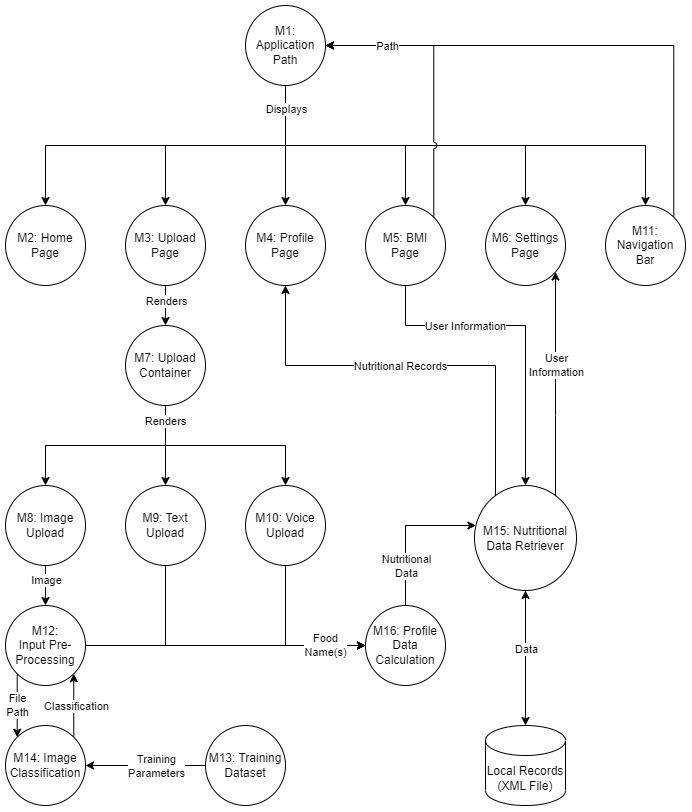
\includegraphics[scale=0.75]{componentdiagram.jpg}

\subsection{Connection Between Requirements and Design} \label{SecConnection}

\wss{The intention of this section is to document decisions that are made
  ``between'' the requirements and the design.  To satisfy some requirements,
  design decisions need to be made.  Rather than make these decisions implicit,
  they are explicitly recorded here.  For instance, if a program has security
  requirements, a specific design decision may be made to satisfy those
  requirements with a password.}

\section{System Variables}

\wss{Include this section for Mechatronics projects}

\subsection{Monitored Variables}

N/A

\subsection{Controlled Variables}

N/A

\subsection{Constants Variables}

N/A

\section{User Interfaces}

\wss{Design of user interface for software and hardware.  Attach an appendix if
needed. Drawings, Sketches, Figma}

\section{Design of Hardware}

\wss{Most relevant for mechatronics projects}
\wss{Show what will be acquired}
\wss{Show what will be built, with detail on fabrication and materials}
\wss{Include appendices as appropriate, possibly with sketches, drawings, CAD, 
etc}

N/A

\section{Design of Electrical Components}

\wss{Most relevant for mechatronics projects}
\wss{Show what will be acquired}
\wss{Show what will be built, with detail on fabrication and materials}
\wss{Include appendices as appropriate, possibly with sketches, drawings,
circuit diagrams, etc}

N/A

\section{Design of Communication Protocols}

\wss{If appropriate}

Front/Backend

\section{Timeline}

\wss{Schedule of tasks and who is responsible}

\bibliographystyle {plainnat}
\bibliography{../../../refs/References}

\newpage{}

\appendix

\section{Interface}

\wss{Include additional information related to the appearance of, and
interaction with, the user interface}

\section{Mechanical Hardware}

N/A

\section{Electrical Components}

N/A

\section{Communication Protocols}

\section{Reflection}

The information in this section will be used to evaluate the team members on the
graduate attribute of Problem Analysis and Design.  Please answer the following questions:

\begin{enumerate}
  \item What are the limitations of your solution?  Put another way, given
  unlimited resources, what could you do to make the project better? (LO\_ProbSolutions)
  \item Give a brief overview of other design solutions you considered.  What
  are the benefits and tradeoffs of those other designs compared with the chosen
  design?  From all the potential options, why did you select documented design?
  (LO\_Explores)
\end{enumerate}

\end{document}